\section{Regression Analysis}
In statistical modeling, regression analysis is a set of statistical processes 
for estimating the relationships between a dependent variable (often called the 
'outcome variable') and one or more independent variables 
(often called 'predictors', 'covariates', or 'features'). 
\cite{enwiki:regressionanalysis} Recall from chapter 1 that 
given a variable $X$ with a continious variable $Y$ 
and a set of observations $D$, a decision function $f$ must be estimated 
that is able to capture the true state of nature and correctly use $X$ to 
predict the corresponding value of $Y$.  

\begin{equation*}
    \underset{X,Y \in D}{f: X \rightarrow Y}
\end{equation*}

The equation above is a general equation for how regression models relates the
independent variables $X$ and the outcome variable $Y$. Though the exact
implementation of the model of this relationship varies throughout different 
methods. One of which we will discuss in this chapter, linear regression.

\section{Solving Linear Regression}
For Ordinary Least Squares (OLS) there exists a closed-form solution to 
calculate the solution parameters. Given a feature matrix $X$ and outcome vector
$Y$ and minimisation of squared errors, the solution parameter matrix $\theta$ 
is calculated as

\begin{equation*}
    \theta = (X^T X)^{-1}X^T
\end{equation*}

This calculation is done only once and is the optimal solution. But there are 
constraints which will lead us to use a gradient descent approach instead.
According to \cite{scikit-learn}, the complexity of the analytical solution
is 

\begin{equation*}
    O(n_{\text{samples}} n_{\text{features}}^2)
\end{equation*}

And compare this with the complexity of the Stochastic Gradient Descent approach
is 

\begin{equation*}
    O(kn\bar{p})
\end{equation*}

where $k$ is the number of epochs in the gradient descent, $n$ the number of
samples and $\bar{p}$ the average number of non-zero attributes in the samples.
Plotting the complexity of the two methods agains increasing sample and features
size we get

\begin{figure}[H]
\label{fig:complexity}
\centering
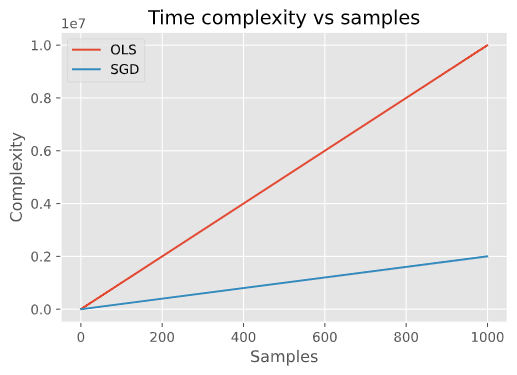
\includegraphics[width=0.45\textwidth]{figures/complexity-samples.png}
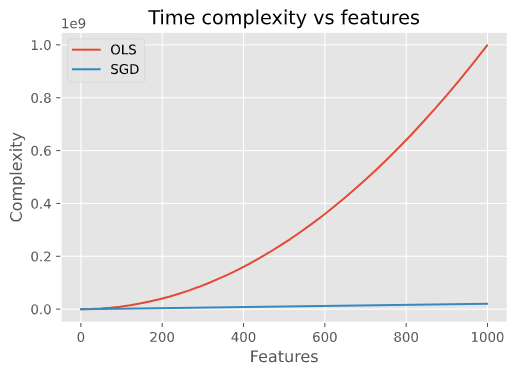
\includegraphics[width=0.45\textwidth]{figures/complexity-features.png}
\caption{Complexities of the two methods.}
\end{figure}

We see that the analytical solution does not handle increasing samples and
especially not increasing features due to the exponential growth in complexity
as features increase. While SGD is much cheaper and robust. For big data 
tasks, using gradient descent is almost always the least demaning way of getting
a solution to the problem.

\section{Notation}
\begin{itemize}
    \item $m = $ The number of training examples
    \item $x = $ The input variables / features
    \item $y = $ The output variable/"target" variables
    \item $(x_i, y_i) = $ A specific example ($i_{th}$ training example)
\end{itemize}

Passing the features into a learning algorithm that outputs a function (denoted $h = $ hypothesis), resulting in the function:
\[
    h_\theta(x) = \theta_0+\theta_1 x
\]
where $\theta_i$ are parameters, $\theta_0$ is the zero condition, and $\theta_1$ is the gradient.

\section{Cost Function}
Recall from the decision tree section on decision trees and regression trees.
There we somehow need to mathematically describe information and how much 
information the model is able to explain. In regression trees we used variance.
Since a model that contains a lot of information about the true state of nature
will have a low variance in it's predictions. A cost function that lets us 
figure out how to fit the best linear prediction line is needed.
We want to solve a minimization problem where we minimize $(h_\theta(x)-y)^2$.

The most common cost function is the mean squared error (MSE):
\[
    J(\theta_0, \theta_1) = \frac{1}{m}\sum_{i=1}^m\left(h_\theta(x_i)-y_i\right)^2
\]

Note that multiplying the cost function by $\frac{1}{2}$ does not change the location of the minima, which is why we use it to form the following cost function:
\bigskip

One half mean squared error:
\[
    J(\theta_0, \theta_1) = \frac{1}{2m}\sum_{i=1}^m\left(h_\theta(x_i)-y_i\right)^2
\]

The cost function determines the parameters, and the values associated with the parameters determine how the hypothesis behaves.
Different values generate different hypotheses.

The MSE cost function is convex.

Finding the global minima in linear regression can be done with a gradient descent algorithm.

\subsection{Cost Function for Multiple Variables}
\[
    J(\theta_0, \theta_1, \cdots, \theta_n) = \frac{1}{2m}\sum_{i=1}^m\left(h_\theta(x_i)-y_i\right)^2
\]

\section{Batch Gradient Descent Algorithm (BGD)}
\begin{itemize}
    \item In each step you look at all the training data
\end{itemize}

\subsubsection{Progress}
\begin{enumerate}
    \item Start with initial guesses, i.e. $(0, 0)$
    \item Keep changing $\theta_0$ and $\theta_1$ a little bit to reduct $J(\theta_0, \theta_1)$
    \item Each time the parameters change, select the gradient which reduces $J(\theta_0, \theta_1)$ the most
    \item Repeat until we converge to a local/global minima
\end{enumerate}
Different starting points will often result in different minimas.

\subsubsection{Formal progress}
\begin{itemize}
    \item Do the following until convergence:
    \begin{itemize}
        \item $\theta_j:=\theta_j-\alpha\frac{\partial}{\partial\theta_j}J(\theta_0, \theta_1)$
        \item For $j=0$ and $j=1$ in this example.
    \end{itemize}
    \item $\alpha$ is the learning rate
    \item $\alpha$ controls how aggressive the gradient descent is
\end{itemize}

"For $j=0$ and $j=1$" means that we update both parameters simultaneously. This is done by first solving the derivative for $\theta_0$ and storing it in a temporary variable. Do the same for $\theta_1$, and then update the original $\theta_j$-values.

\subsubsection{Partial Derivatives}
\[
    \frac{\partial}{\partial \theta_j}J(\theta_0, \theta_1) = \frac{\partial}{\partial\theta_j}\frac{1}{2m}\sum_{i=1}^m(\theta_0+\theta_1x_i-y_i)^2
\]
\[
    \frac{\partial}{\partial \theta_0}J(\theta_0, \theta_1) = \frac{1}{m}\sum_{i=1}^m(\theta_0+\theta_1x_i-y_i)*1
\]
\[
    \frac{\partial}{\partial \theta_1}J(\theta_0, \theta_1) = \frac{1}{m}\sum_{i=1}^m(\theta_0+\theta_1x_i-y_i)x_i^{(1)}
\]
\[
    \frac{\partial}{\partial \theta_j}J(\theta_0, \cdots, \theta_n) = \frac{1}{m}\sum_{i=1}^m(\theta_0+\cdots+\theta_nx_i-y_i)x_i^{(j)}
\]

\subsection{Gradient Descent in Practice}
\begin{itemize}
    \item Feature Scaling (normalize)
    \begin{itemize}
        \item Problems with multiple features should be scaled to a more even scale across the features.
        \item One common way is to use the mean to scale all data into the range $\left[-1, 1\right]$.
        \item Try to create a range between $\left[-3, 3\right]$ and $\left[-\frac{1}{3}, \frac{1}{3}\right]$.
        \item This is done by $x_i = \frac{x_i-\hat{x}}{max(x)-min(x)}$
    \end{itemize}
    \item Running gradient descent on this kind of cost function can take a long time to find the global minima.
\end{itemize}

\section{Practical Tips}
\begin{itemize}
    \item Plot $min(J(\theta))$ with the number of iterations to clearly illustrate the convergence.
    \item Start with a low learning rate, and gradually increase it. It is normal to go for roughly treefold increments (multiply by 3).
    \item We could also use a polynomial regression on the form $(\theta_0 + \theta_1x + \theta_2x^2)$.
\end{itemize}
